\makeheading{Lecture 15 | 2020-11-02}
\section{Residual Plots for Linear Regression Assumptions}

Recall: $ \symbf{Y}=X \symbf{\beta}+\symbf{\varepsilon} $
where $ \symbf{\varepsilon}\sim \Mvn{0,\sigma^2I_{n}} $.
Practically, this means
\[ \varepsilon \stackrel{\text{iid}}{\sim}\N{0,\sigma^2} \]
\begin{itemize}
      \item Independence among all error terms
      \item Normally distributed
      \item Since $ \E{Y_i}=\beta_0+\beta_1x_{i1}+\cdots+\beta_p x_{ip} $
            is implied by $ \E{\varepsilon_i}=0 $ for any
            $ x_{i1},\ldots,x_{ip} $, the linear model
            is appropriate; that is, it correctly explains response
            on average.
      \item Constant error variance $ \sigma^2 $
\end{itemize}
We could assess these assumptions
via $ \varepsilon_i $'s, but we can't observe
$ \varepsilon_i $ directly. Rather, we do have an approximation
via residuals $ e_i $ from the fitted model.

Recall, $ \symbf{e}\sim \Mvn{0,(I-H)\sigma^2} $.
So $ \symbf{e} $ and $ \symbf{\varepsilon} $ are related:
\[ \symbf{e}=\symbf{Y}-X \hat{\symbf{\beta}}=(I-H)\symbf{Y}=
      (I-H)(X \symbf{\beta}+\symbf{\varepsilon})=
      (X \symbf{\beta}-H X\symbf{\beta})+(I-H)\symbf{\varepsilon}=
      (I-H)\symbf{\varepsilon} \]
Note: we can't ``solve'' $ \symbf{\varepsilon} $
since $ (I-H) $ is not invertible since it is not full rank:
recall $ H $ and $ (I-H) $ are idempotent, so
\[ \tr{H}=p+1=\rank{X} \]
\[ \tr{I-H}=n-(p+1)<n \]
Similarly, this does not imply $ \symbf{Y}=\symbf{\varepsilon} $.
So, $ e_i=\varepsilon_i-\sum_{j=1}^{n} h_{ij}\varepsilon_j $
which means $ e_i $ is a good approximation to $ \varepsilon $
when entries of $ h_{ij} $ of $ H $ are small
(which is ``usually'' the case, especially when $ n $ is large).
\[ e_i \sim \N{0,\sigma^2(1-h_{ii})}\iff
      \frac{e_i-0}{\sigma\sqrt{1-h_{ii}}} \sim \N{0,1} \]
If we plug in $ \hat{\sigma} $, that defines
the studentized residuals.
\[ d_i\equiv \frac{e_i}{\hat{\sigma}\sqrt{1-h_{ii}}}  \]
Common practice is to use $ \symbf{e} $ for
the following residual plots/diagnostics,
(using $ d_i $ is also possible) to check model assumptions:

Plot $ \symbf{e} $ versus $ \hat{\symbf{\mu}} $ which
was shown in A2 were mutually independent
since they are multivariate normal with covariance 0.

Typical ``good'' scatter plot will have a random scatter
around $ y=0 $ (no visible patterns).

Problematic scatter plot is when
variance of $ e_i $ is not constant (cone)
increases with fitted values.

In general, plot of $ \symbf{e} $ and $ \hat{\symbf{\mu}} $
can show deviations from independence, constant variance if those
assumptions are violated.

Plot $ \symbf{e} $ versus $ \symbf{x}_j $ for each $ j=1,\ldots,p $
in model when not many predictors. This can help detect non-linearity
between $ \symbf{x}_j $ and $ \symbf{y} $, not as practical when
$ p $ is large.

Typical ``good'' scatter plot will have a random scatter
around $ y=0 $ (no visible patterns).

If the observation numbers were collected in some order
(time, space, etc.), also plot $ e_i $ versus indices
$ i $ to check for any patterns (again, look for random scatter)

Histogram of $ \symbf{e} $: is it bell shaped and symmetric
to assess Normal assumption, but the histogram can't easily
detect overly fat/thing tails.

Q-Q plot of $ \symbf{e} $ more formally assess Normality:
scatter plot of ordered quantiles from 2 distributions.
In our case: empirical quantiles from residuals (data)
versus theoretical quantiles from assumed Normal distribution.
If quantiles roughly match, the points will roughly fall
on the $ 45^\circ $ line through origin.

If these sets of residuals plots show violations, then that could
affect the validity of confidence intervals, hypothesis tests, etc.

\subsection{R Demo}
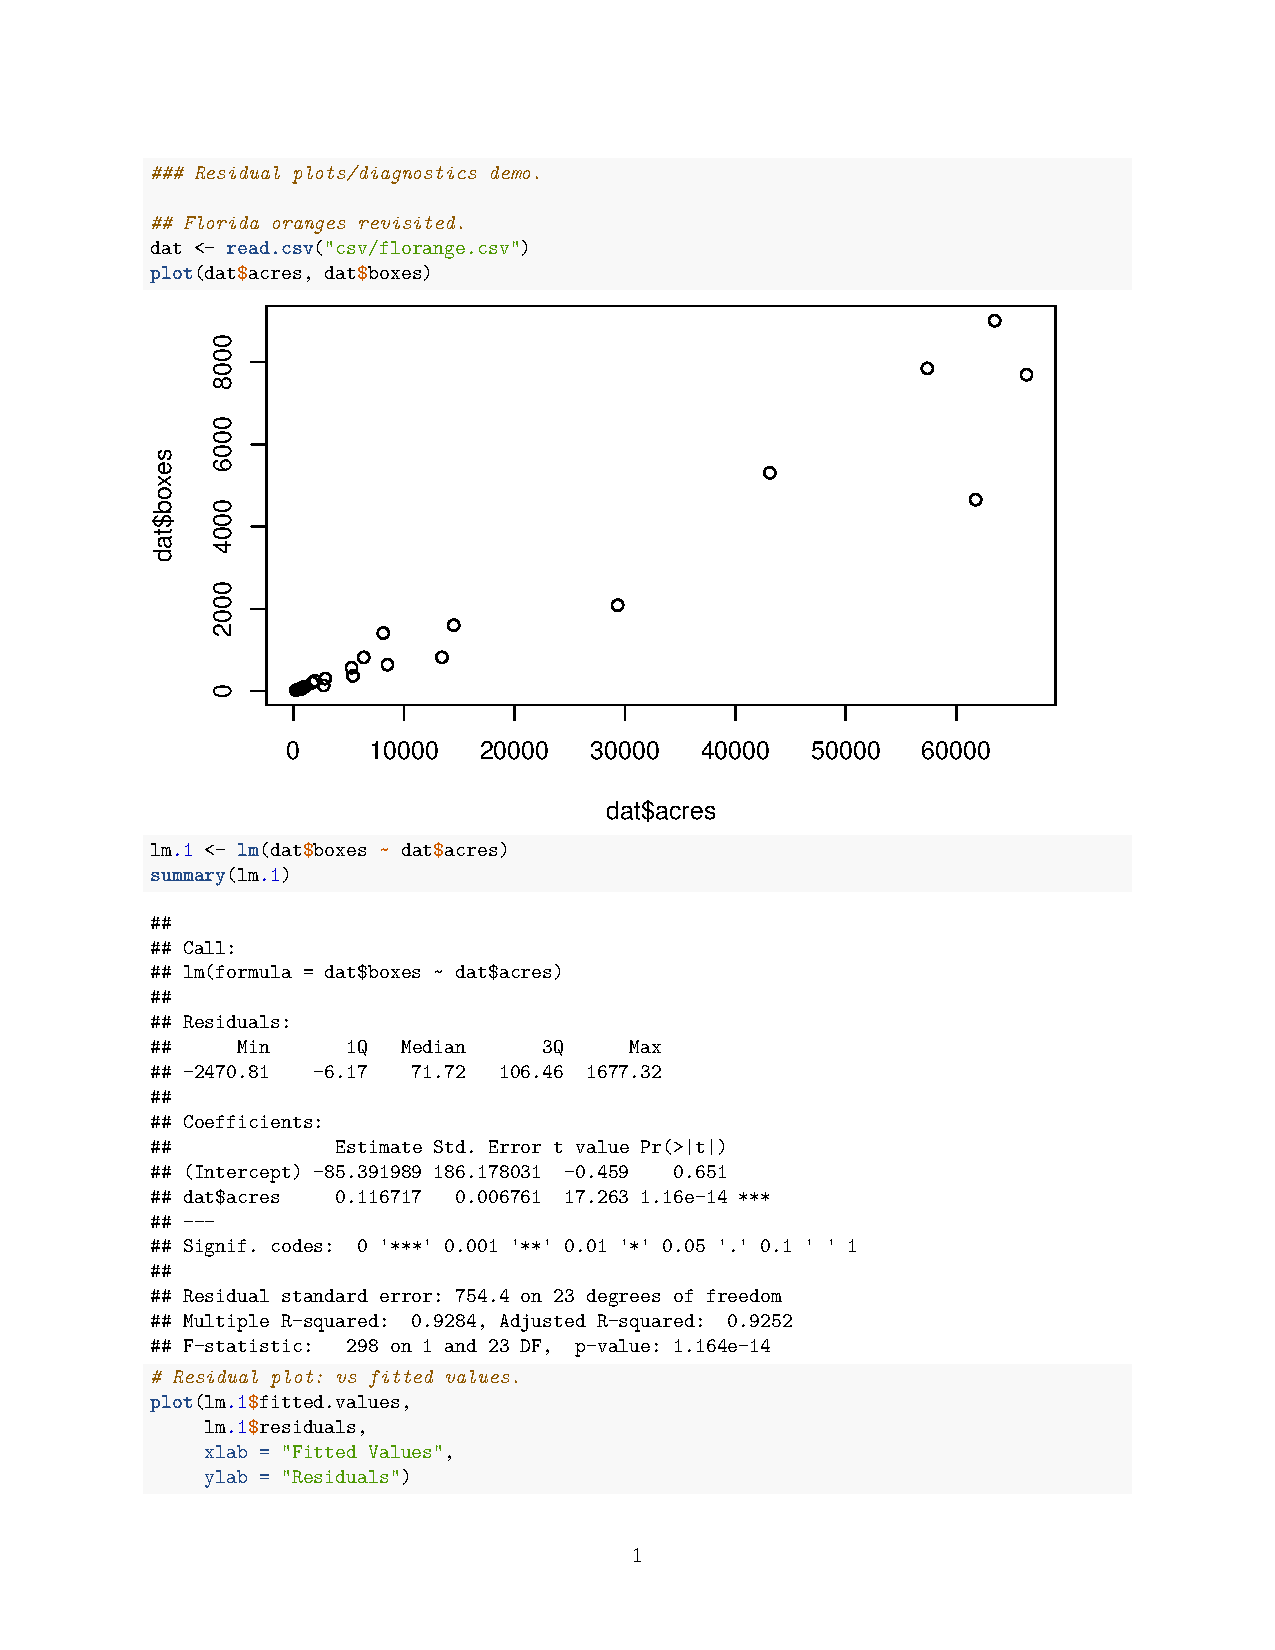
\includepdf[pages=-]{lec_15-demo.pdf}
